\section{LSTM}
\label{section:Method:LSTM}

% Train val split
%When working with time series it is important to think about how one splits up
%the dataset into training, validation, and test set.
%One key aspect when forecasting a time series is the newer the information,
%the more relevant it is for the forecast.
%In a perfect world the model will be able to use all the available data for training,
%right up to the point of forecast, then try to forecast the wanted horizon.
%However, in order to tune hyperparameters and avoid overfitting to the training
%set, we need a validation set.

% In a stateful LSTM everything fed through the network is seen by the network
% as follow each other in time. Since the validation step is executed at the end of
% each epoch, and each epoch pass feeds all the training data through the network,
% it makes sense to use the last section of the training data as the validation data.


The LSTM consisted of $n$ layers of stacked LSTM cells followed by a
dense layer with the same output size as our forecast horizon.
The parameters used for the LSTM cells are listed in \Cref{table:LSTM-cell-parameters}
and the parameters used in the dense layer is listen in \Cref{table:LSTM-dense-cell-parameters}.

\begin{table}[h]
  \centering
  \caption{LSTM cell parameters. Values with a T value was tuned}
  \label{table:LSTM-cell-parameters}
  \begin{tabular}{|l|l|}\hline
    Parameter              & value             \\ \hline
    \hline
    units,                 & T                 \\
    activation             & "tanh"            \\
    recurrent\_activation  & "sigmoid"         \\
    use\_bias              & True              \\
    kernel\_initializer    & "glorot\_uniform" \\
    recurrent\_initializer & "orthogonal"      \\
    bias\_initializer      & "zeros"           \\
    unit\_forget\_bias     & True              \\
    kernel\_regularizer    & None              \\
    recurrent\_regularizer & None              \\
    bias\_regularizer      & None              \\
    activity\_regularizer  & None              \\
    kernel\_constraint     & None              \\
    recurrent\_constraint  & None              \\
    bias\_constraint       & None              \\
    dropout                & T                 \\
    recurrent\_dropout     & T                 \\
    return\_sequences      & False             \\
    return\_state          & False             \\
    go\_backwards          & False             \\
    stateful               & True              \\
    time\_major            & False             \\
    unroll                 & False             \\
    \hline
  \end{tabular}
\end{table}

\begin{table}[h]
  \centering
  \caption{LSTM dense parameters}
  \label{table:LSTM-dense-cell-parameters}
  \begin{tabular}{|l|l|}\hline
    Parameter             & value                \\ \hline
    \hline
    units                 & outout\_window\_size \\
    activation            & None                 \\
    use\_bias             & True                 \\
    kernel\_initializer   & "glorot\_uniform"    \\
    bias\_initializer     & "zeros"              \\
    kernel\_regularizer   & None                 \\
    bias\_regularizer     & None                 \\
    activity\_regularizer & None                 \\
    kernel\_constraint    & None                 \\
    bias\_constraint      & None                 \\
    \hline
  \end{tabular}
\end{table}

\subsubsection{LSTM Tuning}
The hyperparameters of the LSTM is tuned with the Optuna Python package
with the Bayesian optimal algorithm [\Cref{section:BT:Hyperparameters}].
The hyperparameter minimum and maximum values are shown in \Cref{table:LSTM-hyperparameters-tuning-range}.
These values were carefully chosen after many tuning experiments.
\Cref{fig:lstm:optuna-parameter-slice-figure} show a report from an optuna tuning,
and how diffrent parameter combinations improved the model.

\begin{table}[h]
  \centering
  \caption{LSTM Hyperparameter tuning range}
  \label{table:LSTM-hyperparameters-tuning-range}
  \begin{tabular}{|l|l|}\hline
    hyperparameter       & Tuning range        \\ \hline
    \hline
    hidden\_size         & [1, 100]            \\
    number\_of\_layers   & [1, 2]              \\
    dropout              & [0.0, 0.4]          \\
    recurrent\_dropout   & [0.0, 0.4]          \\
    optimizer\_name      & ['RMSprop', 'Adam'] \\
    learning\_rate       & [1e-7, 1e-2]        \\
    number\_of\_epochs   & [1, 40]             \\
    batch\_size          & [32, 32]            \\
    input\_window\_size  & 10                  \\
    output\_window\_size & 7                   \\
    number\_of\_features & 1                   \\
    number\_of\_trials   & 200                 \\
    stateful\_lstm       & true                \\
    \hline
  \end{tabular}
\end{table}
\begin{figure}[h!]
  \centering
  \caption{A Optuna generated SLICE plot showing model perfomance with different hyperparameter combinations.}
  \begin{subfigure}[0]{\textwidth}
    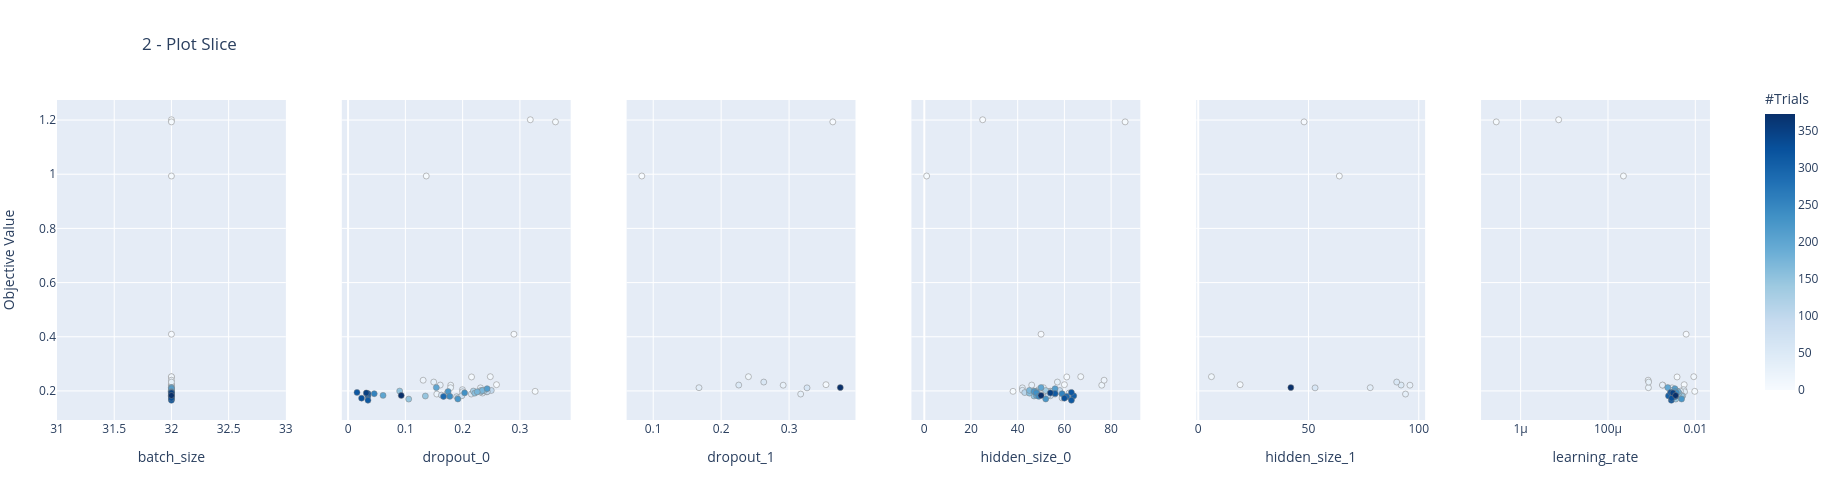
\includegraphics[width=\textwidth]{./figs/hyperparameter_plot_ranges_dataset2(0).png}
    \hfill
    \caption{First 6 hyperparameters}
  \end{subfigure}
  \begin{subfigure}[0]{\textwidth}
    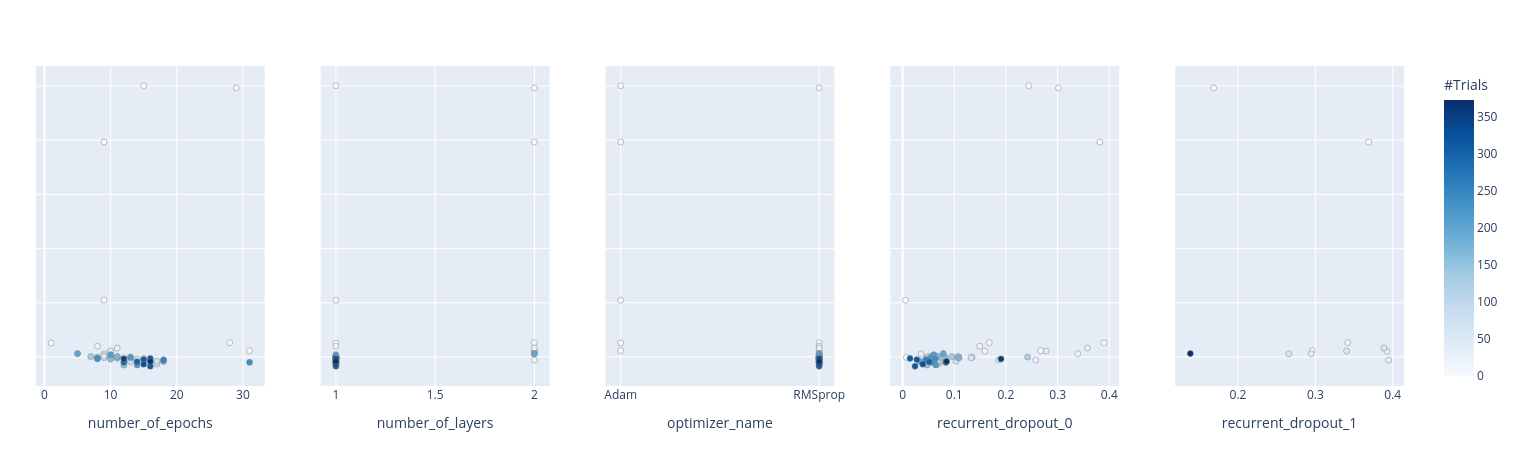
\includegraphics[width=\textwidth]{./figs/hyperparameter_plot_ranges_dataset2(1).png}
    \hfill
    \caption{Last 5 hyperparameters}
  \end{subfigure}
  \label{fig:lstm:optuna-parameter-slice-figure}
\end{figure}

\subsubsection{Stateful LSTM and hidden states}
\label{section:Method:stateful-lstm-and-hidden-states}
%One can argue that a stateless LSTM which resets its state before each batch
%can mimic a stateful LSTM with a sufficiently large enough batch size.
%After some prototype testing we concluded that an stateful LSTM
%was superior for our problem.
%TODO[Insert spreadshit data with testing results.]

Intuitively the problem at hand requires a stateful LSTM [\cref{section:BT:stateful-vs-stateless}].
One problem with stateful LSTMs is that they require all the input to have the same
batch size.
This is because the two-state vectors $h_t$ and $c_t$ have the shape
$(batch\_size, input\_length, features)$. In a stateless LSTM, these
vectors are initialized with zero values at the beginning of each forward pass,
so the $batch\_size$ can be inferred from the input.
In a stateful LSTM, these vectors are initialized once together with the rest
of the network, and so the $batch\_size$ needs to be specified with
the rest of the hyperparameters.

As a consequence the training data, validation data, and test data all
need to use the same $batch\_size$, which is problematic.
The easiest solution is to use online learning, by setting the batch size to 1.
However, this means calculating gradients and doing a backpropagation for each
timestep in our dataset, which is highly inefficient.

A batch size bigger than one means that the number of samples in
the training data and validation data and test data has to all be
dividable by the batch size. If not the last batch will have too few samples in it,
and the network will reject it.
The most common solution is to find the highest common factor
between the training data and the test data, and use that as batch size.
This is not a solution that works on this problem because in our global model
we train our model on many different time series of different lengths,
and
also, our test data consists of exactly 1 sample with a size equal the
forecasting horizon, per time series.
We managed to solve the test data problem by creating two models with
different batch sizes. We trained the first model on the training data,
then copied the internal weights over to the second model, which had a
batch size of one, for testing and
predictions.

The solution of copying weights was not available for the validation data
because the validation step in Keras is incorporated into the training function.
Due to time constraints, we did not want to dive deep into the Keras internals
to see if it was possible to solve this problem by hand.

Our solution ended up being to remove a number of samples at the beginning of
the dataset in order to make the total number of samples dividable by the batch size,
and then make the validation set equal to one batch. Removing data from the beginning,
seemed obvious as newer data will have more relevance than older data.
This meant that we also had to remove batch size as a tunable hyperparameter,
because the model would favor lower batch sizes because that meant fewer validation data batches,
which equals potentially fewer examples to get wrong.

Instead of automatically tuning batch sizes, we did some manual testing, and
ended up setting batch size 32 for all experiments.


\subsubsection{Reset states}
Since  the hidden states are never reset automatically in Keras stateful LSTM
we had to do it ourselves.

\textbf{Local models}

For the local models, we are resetting the internal state at the beginning
of each epoch as well as before testing. We do not reset states before validation,
because the validation step always comes after an epoch run, and the
validation data are taken from the end of the training data for each time series.
This means the model will in fact have the correct hidden state when starting the validation step.

During testing, we have to be a bit more clever. We ran the whole training set plus
the validation set through the networks prediction loop before predicting the test
set and calculate test metrics.
This is for the model to "see" the whole picture and have the correct
internal state before predicting the test set.
Neptune experiment \textit{MAS-396} and \textit{MAS-397} confirms
that this tactic pay off. MAS-397 achieved a MAS score of $2.00$ on the test set
without resetting states and passing through training and validation data before
the test set. In MAS-396 we used the exact same setup, but with resetting states
before the test set. MAS-396 achieved a MAS score of $1.67$.

\textbf{Global models}
For global models, we followed the concept presented by \cite{Smyl2020},
with global weights, but local states.

As described in [TODO: WHere we describe the pipeline behind the global models]
we concatenate multiple time series after one another during the training of a global model.
This means we have to reset the hidden state during the training of a global model
or else we will give our model a false sense of dependencies between
the independent time series.

%Our fix to this solution is not perfect, and might be an area worth critique.
As described in \Cref{section:Method:issues-lstm:fixed-batch-size} all
batches had to be the same size. Our time series was concatenated one after
each other into one large time series.
Our fix was to pass in a lambda callback to Keras which ran after each batch.
We counted how many batches it would need to fit each time series.
We counted how many batches it had ran. When the number of batches ran equals
the number of batches in a time series we reset the hidden state.
One flaw, however, is that since it is possible for one batch to
contain two time series, it might not reset the hidden state at the exact
right time, but in the worst-case scenario a $batch\_size - 1$ number of
samples too late. Still, this technique did prove to be successful.
Neptun experiment \textit{MAS-491} achieved a MASE metric of \textbf{19.61}
without reseting states during training.
Neptum experiment \textit{MAS-492} achieved a MASE metric of \textbf{2.36}.

Below is a simplified pseudo code for the algorithm which resets hidden states
during training.
\begin{enumerate}
  \item time\_series\_counter = 0
  \item time\_series\_number\_of\_batches\_list = [TS.length() // batch size for each TS in time-series ]
  \item start\_training\_loop()
  \item after each batch: if current batch number ==
        time\_seires\_number\_of\_batches\_list[time\_series\_counter]
        then -\> reset\_hidden\_state()
  \item time\_series\_counter += 1
\end{enumerate}




% Tuning: How did we specify tuning ranges

% Model choice: 

% Hvordan har vi valgt å tune med trening og test set

% Global model, how did we train on multiple dataset?